
\section{Achieving efficient elasticity}
\label{sec:design}

\subsection{In-memory data organization}
\label{sec:data_organization}

This section presents the design and implementation of the mechanisms that enable efficient and minimally disruptive elasticity in \OurImplementation{}. 
We first describe the in-memory data organization, focusing on how \OurImplementation{}'s RDMA-friendly memory allocator ensures that logical data groupings (slots) are reflected in the physical memory layout, 
enabling efficient high-speed data transfers (Section~\ref{sec:data_organization}). We then detail the migration protocol,
outlining how \OurImplementation{} orchestrates seamless and transparent data migrations across nodes while continuing to serve client requests (Section~\ref{sec:migration-protocol}). 
A key part of the migration process is the index update, which integrates transferred key-value pairs into the destination’s serving data structures (Section~\ref{sec:index_updating}).

Building upon this foundation, we improve upon the base migration protocol by overlapping computation and communication for better resource utilization (Section \ref{sec:groups-stages}). 
Finally we introduce a self-regulating mechanism that allows \OurImplementation{} to preserve client workload performance even during intensive migration phases (Section \ref{sec:throttling}).

\begin{figure}
	\centering
	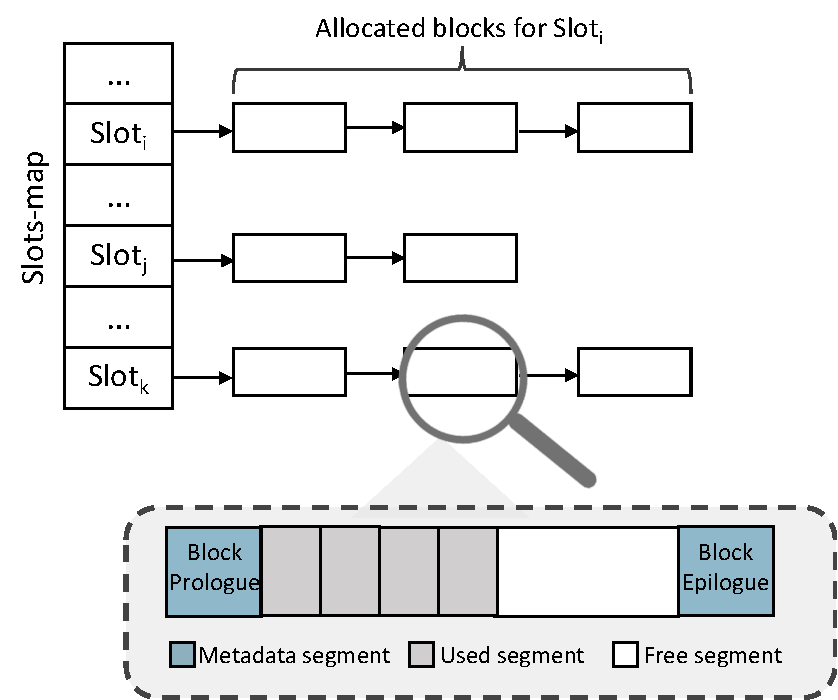
\includegraphics[width=0.8\columnwidth]{illustrations/allocator/allocator_data_organization.pdf}
	\caption{Allocator internal data organization}
	\label{fig:allocator_organization}
\end{figure}

\begin{figure*}[t]
	\centering
	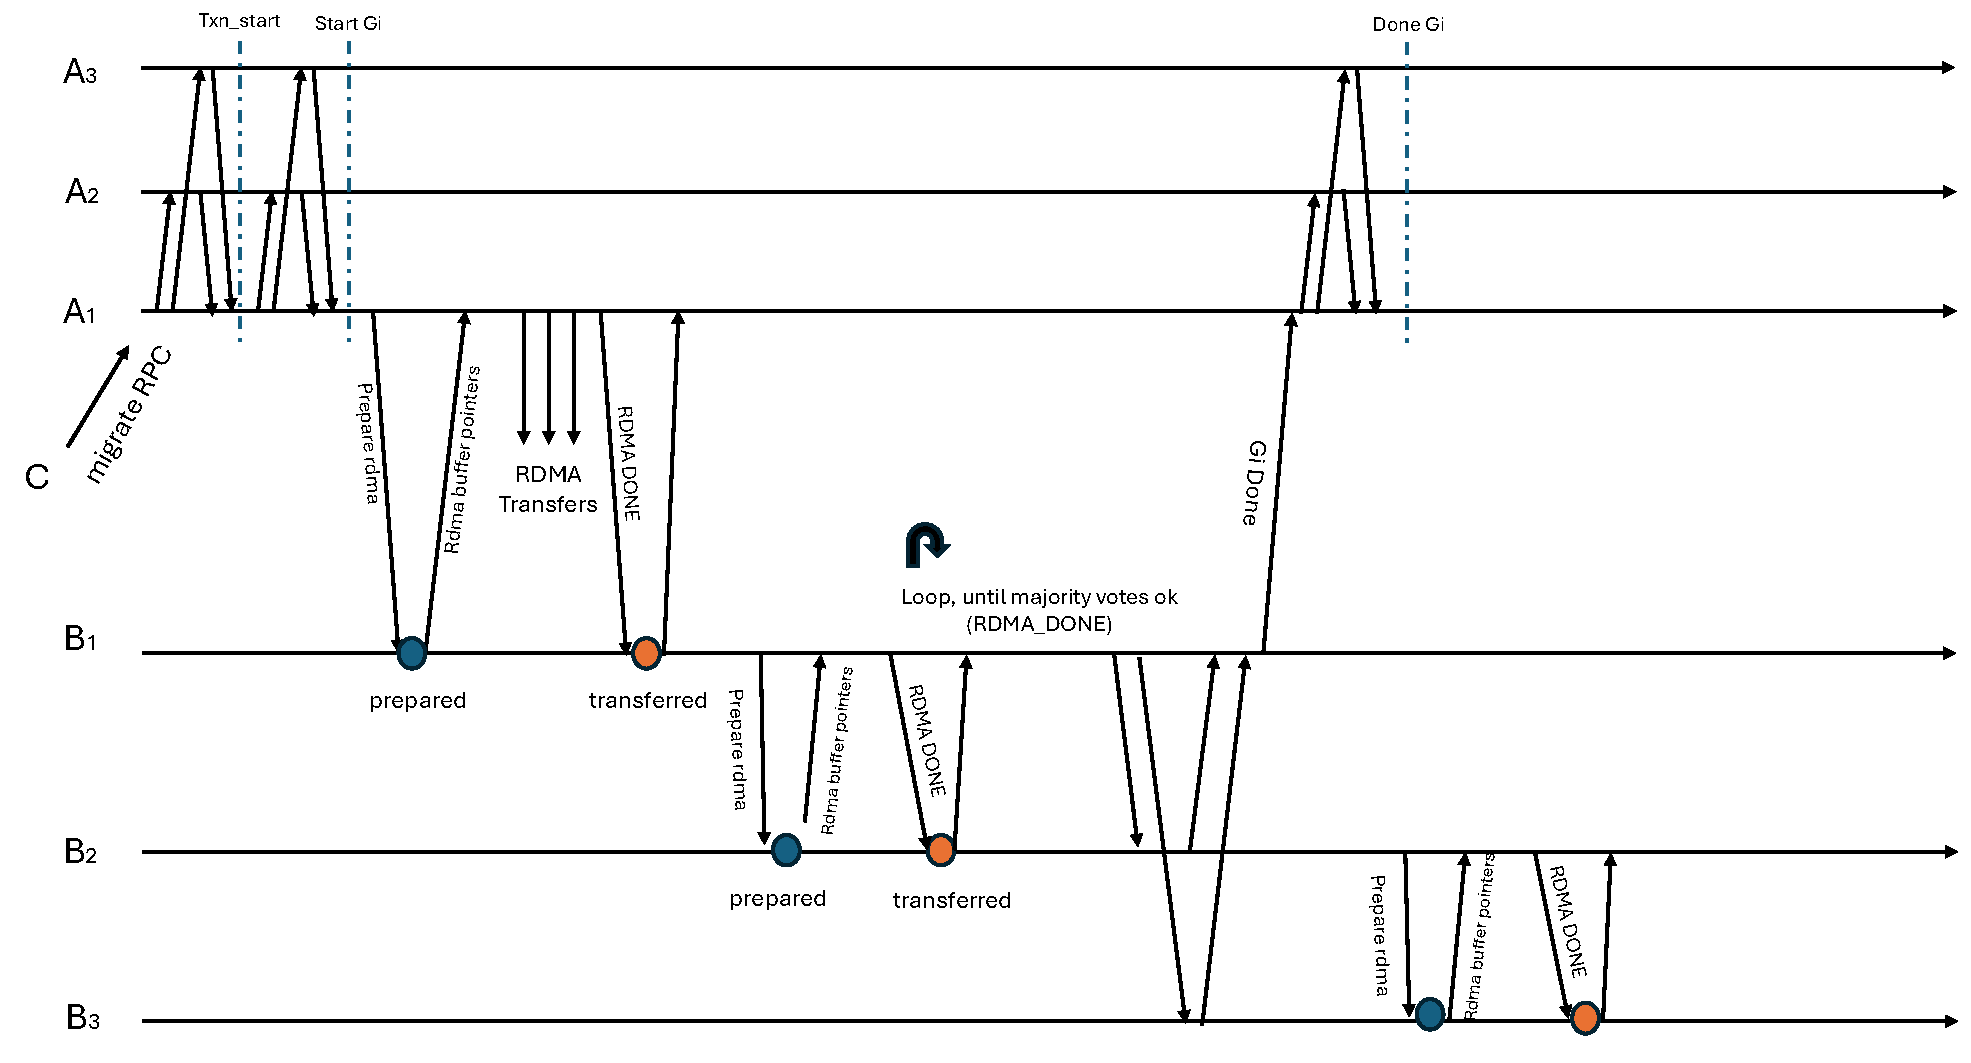
\includegraphics[width=0.9\textwidth]{illustrations/migration_flow/protocol.pdf}
	\caption{\OurImplementation{} baseline migration protocol}
	\label{fig:migration_flow}
\end{figure*}

Key-value stores (KVSs) typically organize data in logical partitions called {\em shards}, {\em slots}, or {\em tokens} in different systems~\cite{mongodb,redis-pure,cassandra-paper}. 
In this paper, we uniformly refer to them as \emph{slots}, regardless of the underlying system.

In most KVSs today, in-memory data organization does not necessarily align with the logical organization of data (i.e., slots).
The reason is that general-purpose memory allocators typically disregard the logical affinity between KV pairs, leading to data of the same slot being scattered across different memory locations within a node. Consequently, during data migrations, a node must gather scattered memory buffers to transfer a slot, resulting in long \emph{gather} lists for RDMA operations. 
Such long RDMA chains of small buffers are inefficient, severely degrading transfer bandwidth and efficiency.

To address this, \OurImplementation{} introduces a bulk-transfer-oriented, RDMA-friendly memory allocator that ensures in-memory layouts mirror the logical slot structure.
Upon a memory allocation request, \OurImplementation{}’s allocator, leveraging the knowledge of which slot ID each key-value pair belongs to, aims to place all data of a slot into contiguous physical memory regions. 

The allocator maintains metadata in the form of a hash table, where each bucket represents a distinct slot (Fig.~\ref{fig:allocator_organization}).
Since it is challenging to predict all records and their memory requirements for each slot without prior knowledge of the dataset, the allocator operates using fixed-size memory regions called \emph{blocks}.
Records within a slot are packed across one or more blocks. When a block becomes full, a new one is allocated to continue storing the slot's data.
Each block includes metadata \emph{prologue} and \emph{epilogue} to efficiently keep track of the block boundaries as well as the used and free segments in it.

We replace the generic memory allocation policy with our tailored allocator.
Each memory allocation request is tagged with its associated slot, allowing the allocator to co-locate key-value pairs belonging to the same slot.

The allocator is a full-featured memory manager that supports all standard operations, including inserts, deletes, and updates.
To efficiently manage memory reuse, it employs a free list to track available memory regions, enabling fast identification of suitable space for new allocations.
Additionally, it supports coalescing adjacent free regions to reduce fragmentation and improve overall space utilization.

For every inserted record, the allocator adds a metadata header that records the segment boundaries and includes padding to ensure proper alignment to double word (8 bytes) boundaries.
This allows to use the least significant bits of the memory address (that we assume it is zero due to alignment) to encode addition metadata (e.g. the status of the segment).

During the migration process, when a node offloads certain slots to another node, it can request a list of memory blocks associated with those slots.
This slot-aware memory organization substantially reduces the number of descriptors in RDMA operations (i.e., shorter gather lists composed of larger buffers), leading to significantly improved RDMA performance.
Furthermore, communicating through fewer, larger memory regions (MRs) optimizes memory \emph{registration} overhead\footnote{RDMA operations require that memory regions (MRs) be {\em registered} with RNICs, assigning them Remote Keys (RKeys) used in remote access}.
RDMA-capable NICs (RNICs) can more efficiently manage memory resources when buffers are contiguous, allowing for more efficient use its memory management resources (e.g., consume fewer entries as data in \OurImplementation{} is better packed, or by coalescing entries when contiguous).
Overall, \OurImplementation{}'s memory organization greatly enhances the efficiency of bulk slot transfers critical for rapid elasticity.




\subsection{Fault Model}
We assume a fail-stop failure model, 
in which nodes may crash and permanently stop executing. 
A crashed node does not recover unless explicitly restarted.


The migration protocol guarantees no data loss as long as at least one replica remains alive in each involved replication group, and it tolerates failures according to the Raft failure model. If failures occur mid-migration, the protocol can resume from the last successfully committed epoch without requiring a full restart, ensuring both safety and efficiency.

The system employs synchronous replication for write operations using a Raft. 
Each replication group consists of a fixed number of nodes, where one node acts as the leader and the remaining nodes act as replicas. 
A write is considered committed only after it has been durably replicated to a majority of the nodes in the replication group.

The \OurImplementation{} migration protocol guarantees no data loss provided that at least one replica containing the committed data remains alive in each replication group. 
A failure of both the leader and all replicas that store a particular piece of data results in permanent data loss for that data item. 
Consequently, \OurImplementation{} cannot tolerate the simultaneous crash of all nodes in a replication group.

When nodes are restartable, a recovering node may rejoin the system and re-integrate into a replication group. 


The migration protocol guarantees no data loss as long as at least one replica remains alive in each involved replication group, 
and it tolerates failures according to the Raft failure model. 
If failures occur mid-migration, the protocol can resume from the last successfully committed epoch without requiring a full restart, ensuring both safety and efficiency.


\subsection{Fault Tolerant Migration protocol}
\label{sec:migration-protocol}

The migration protocol is designed to operate concurrently with client requests and relies on Raft for coordination of source and reciepient, 
and one-sided RDMA for efficient bulk data transfer.
Data migrations in \OurImplementation{} are managed by the \emph{Migration Manager (MM)} module, which orchestrates the entire migration process on the source and destination nodes. 
The MM ensures seamless data transfer and coordinates the ownership handover upon successful migration. 
The migration process involves both the transfers of data and its integration into the destination node’s active dataset. 

During migration, there are two replica groups involved.
the \emph{donor} (source) group, which holds the data to be migrated, and the \emph{recipient} (destination) group, 
which will receive and integrate the migrated data. Each group has a leader and followers. The leader coordinates the migration process within its group.

At first, the protocol should transfer the data from the source to the destination (leader-to-leader) and ensure the migrating data can tolerate crashes before stoping the double reads. 
Before stopping the double reads and disconnecting the source replica group for that group, the destination replica group should transfer the data to a majority of replicas (leader-to-replica) 
and integrate the received data into leader recipient recplica's active dataset via index updates (Section~\ref{sec:index_updating}). 
Leader-to-replica on the destination replica group, have two paths. The fast path which the majority of the replicas have received the migrating data. This path must finish before stopping the double reads to ensure that the data is available on a majority of replicas. 
The slow path which the minority of the replicas have not received the data. This can happen asynchronously and can complete after stopping the double reads. 
At some point all nodes will eventually receive the migrated data from either the fast path or the slow path.
Fig.~\ref{fig:migration_flow} provides an overview of \OurImplementation{}’s migration process. 
Migration is initiated by a coordinator $C$, which instructs target source replica leader to start a transaction and migrate a set of slots to a destination replica leader $D$.
The protocol proceeds in subtransactions ($G_i$), each corresponding to a subset of the total slots. 
For each $G_i$, source replica group records the start of $G_i$.
For each group, the source first enters a prepare phase, during which it establishes RDMA buffers and exposes memory regions containing the data to be migrated. 
Buffer metadata, including RDMA pointers and access keys, are disseminated to the destination group via a reliable control path.


Once preparation completes, 
the source leader performs one-sided RDMA WRITE operations to write data directly from the source leader replica to the destination side replica leader. 
Upon a transfer completion of a group $G_i$, the source leader issues an RDMA\_DONE acknowledgment.


To ensure correctness under failures, the protocol requires a majority acknowledgment within the destination replication group before marking a batch as successfully transferred. 
Since the majority of replicas in the destination group must confirm that received the data, the protocol guarantees that at least one replica will have the complete data even in the event of failures, therefore clients can safely ask and proceed to the next group.
At this point, the group is marked as completed (Gi Done) and committed via Raft on source replication group.

During migration of a group, writes are directed to the destination replica group, while reads may be served from either the source or destination group, depending on the migration state of the accessed data.
This guarantees that no committed updates are lost. 



After all groups complete, a transaction is considered complete and can safely cleanup the transaction state. 









\subsection{Index updating}
\label{sec:index_updating}


Transferring data using RDMA enables the source node to write data directly into the target node’s memory.
However, transferring raw data alone is insufficient. 
In \OurImplementation{}, a dictionary-like data structure serves as an index, maintaining pointers to the actual key-value pairs. 
Therefore, after the data transfer completes, the dictionary is updated to reflect the new memory locations—a process referred to as the \emph{index update}.

\OurImplementation{} handles index updates using dedicated background threads with lower scheduling priority to minimize interference with client-serving operations. 
Since these background threads run concurrently with client threads, multiple threads may access and update the dictionary simultaneously.
To ensure consistency, \OurImplementation{} employs fine-grained locking for dictionary access and modification.

During migration, all new writes are directed to the destination node. Consequently, data received from the source may contain stale versions of keys. As part of the index update, \OurImplementation{} detects and discards these stale entries, 
ensuring that only the most recent values are preserved in the dictionary.



































